\documentclass[12pt]{report}
\usepackage[utf8]{inputenc}
\usepackage[russian]{babel}
%\usepackage[14pt]{extsizes}
\usepackage{listings}
\usepackage{graphicx}
\usepackage{amsmath,amsfonts,amssymb,amsthm,mathtools} 
\usepackage{pgfplots}
\usepackage{filecontents}
\usepackage{float}
\usepackage{comment}
\usepackage{indentfirst}
\usepackage{eucal}
\usepackage{enumitem}
%s\documentclass[openany]{book}
\frenchspacing

\usepackage{array}

\usepackage{verbatim}

\usepackage{caption}
\captionsetup{labelsep=endash}
\captionsetup[figure]{name={Рисунок}}

\usepackage{indentfirst} % Красная строка

\usetikzlibrary{datavisualization}
\usetikzlibrary{datavisualization.formats.functions}

\usepackage{amsmath}


% Для листинга кода:
\lstset{ %
	language=c,                 % выбор языка для подсветки (здесь это С)
	basicstyle=\small\sffamily, % размер и начертание шрифта для подсветки кода
	numbers=left,               % где поставить нумерацию строк (слева\справа)
	numberstyle=\tiny,           % размер шрифта для номеров строк
	stepnumber=1,                   % размер шага между двумя номерами строк
	numbersep=5pt,                % как далеко отстоят номера строк от подсвечиваемого кода
	showspaces=false,            % показывать или нет пробелы специальными отступами
	showstringspaces=false,      % показывать или нет пробелы в строках
	showtabs=false,             % показывать или нет табуляцию в строках
	frame=single,              % рисовать рамку вокруг кода
	tabsize=2,                 % размер табуляции по умолчанию равен 2 пробелам
	captionpos=t,              % позиция заголовка вверху [t] или внизу [b] 
	breaklines=true,           % автоматически переносить строки (да\нет)
	breakatwhitespace=false, % переносить строки только если есть пробел
	escapeinside={\#*}{*)}   % если нужно добавить комментарии в коде
}


\usepackage[left=2cm,right=2cm, top=2cm,bottom=2cm,bindingoffset=0cm]{geometry}
% Для измененных титулов глав:
\usepackage{titlesec, blindtext, color} % подключаем нужные пакеты
\definecolor{gray75}{gray}{0.75} % определяем цвет
\newcommand{\hsp}{\hspace{20pt}} % длина линии в 20pt
% titleformat определяет стиль
\titleformat{\chapter}[hang]{\Huge\bfseries}{\thechapter\hsp\textcolor{gray75}{|}\hsp}{0pt}{\Huge\bfseries}


% plot
\usepackage{pgfplots}
\usepackage{filecontents}
\usetikzlibrary{datavisualization}
\usetikzlibrary{datavisualization.formats.functions}

\begin{document}
	%\def\chaptername{} % убирает "Глава"
	\thispagestyle{empty}
	\begin{titlepage}
		\noindent \begin{minipage}{0.15\textwidth}
			
\includegraphics[width=\linewidth]{inc/b_logo}
		\end{minipage}
		\noindent\begin{minipage}{0.9\textwidth}\centering
			\textbf{Министерство науки и высшего образования Российской Федерации}\\
			\textbf{Федеральное государственное бюджетное образовательное учреждение высшего образования}\\
			\textbf{~~~«Московский государственный технический университет имени Н.Э.~Баумана}\\
			\textbf{(национальный исследовательский университет)»}\\
			\textbf{(МГТУ им. Н.Э.~Баумана)}
		\end{minipage}
		
		\noindent\rule{18cm}{3pt}
		\newline\newline
		\noindent ФАКУЛЬТЕТ $\underline{\text{«Информатика и системы управления»}}$ \newline\newline
		\noindent КАФЕДРА $\underline{\text{«Программное обеспечение ЭВМ и информационные технологии»}}$\newline\newline\newline\newline\newline
		
		\begin{center}
			\noindent\begin{minipage}{1.1\textwidth}\centering
				\Large\textbf{Отчет по лабораторной работе №3}\newline
				\textbf{по дисциплине <<Моделирование>>}\newline\newline
			\end{minipage}
		\end{center}
		
		\noindent\textbf{Тема} $\underline{\text{Генераторы псевдослучайных чисел}}$\newline\newline
		\noindent\textbf{Студент} $\underline{\text{Слепокурова М.Ф.}}$\newline\newline
		\noindent\textbf{Группа} $\underline{\text{ИУ7-76Б}}$\newline\newline
		\noindent\textbf{Оценка (баллы)} $\underline{\text{~~~~~~~~~~~~~~~~~}}$\newline\newline
		\noindent\textbf{Преподаватель} $\underline{\text{Рудаков И.В.}}$\newline\newline\newline
		
		\begin{center}
			\vfill
			Москва~---~\the\year
			~г.
		\end{center}
	\end{titlepage}

\setcounter{page} {2}





\section*{Постановка задачи}
Изучить методы генерирования псевдослучайных чисел и критерии оценки случайности последовательности. Реализовать собственный критерий оценки и проверить его работу на одноразрядных, двухразрядных и трехразрядных последовательностях, полученных табличным и выбранным алгоритмическим методом. Реализовать возможность ручного ввода последовательности чисел и оценки ее случайности по разработанному критерию.

\section*{Теория}
\subsection*{Алгоритмический метод}
В качестве алгоритмического метода генерации псевдослучайных чисел был выбран линейно конгруэнтный алгоритм. Для реализации метода необходимо задать следующие константы:
\begin{itemize}
    \item $m > 0$ --- модуль; 
    \item $0 \leq a \leq m$ --- множитель;
    \item $0 \leq  c \leq m$ --- приращение;
    \item $0 \leq x_0 \leq m$ --- начальное значение.
\end{itemize}

Тогда последовательность можно сгенерировать с помощью реккурентной формулы:
\begin{equation}
    x_{n+1} = (ax_{n}+c)\mod{m}
\end{equation}

Для того, чтобы проверить работоспособность разработанного критерия оценки случайности, в рамках выполнения работы использовались случайно сгенерированные библиотекой начальные значения $m$, $a$, $c$, $x_0$.

\subsection*{Табличный метод}
Для табличного метода была использована таблица некоррелированных случайных чисел из книги <<Million Random Digits with 100,000 Normal Deviates>>. Суть метода заключается в последовательном чтении уже сгенерированной таблицы значений.

\subsection*{Критерий оценки}
Для оценки случайности последовательностей был разработан собственный критерий. В основе созданного критерия лежит оценка частот вхождения элементов последовательности и оценка приращений между соседними элементами.

Для каждого элемента последовательности предварительно вычисляется количество его вхождений в эту последовательность, после чего вычисляется максимальное количество повторяющихся количеств вхождений --- $k$. 

Затем для последовательности вычисляются приращения между ее соседними элементами, после чего вычисляется максимальное количество повторяющихся приращений --- $m$.

Тогда для последовательности длиной $l$ запишем предварительную формулу для вычисления коэффициента:
\begin{equation}
    rate' = \frac{k+m+1}{l} 
\end{equation}

Заметим, что максимальное значение коэффициента = 2, когда $m+1$ и $k$ = $l$. Для того, чтобы коэффициент принимал значения в диапазоне от 0 до 1, необходимо поделить полученное значение на максимальное, т.е. пополам. Получается, чем выше значение коэффициента, тем менее случайна последовательность --- такую оценку сложно воспринимать, поэтому инвертируем полученное значение путем его вычитания из нового максимального значения диапазона, равного единице. 
Примечание: используем значение $m+1$, а не $m$, чтобы получать значение коэффициента 0 для последовательностей, состоящих из одного повторяющегося элемента.

Тогда итоговую формулу для вычисления коэффициента случайности можно записать как:
\begin{equation}
    rate = 1-\frac{k+m+1}{2l} 
\end{equation}


Теперь имеем коэффициент, принимающий значения из диапазона от 0 до 1, причем чем больше значение, тем более случайна рассматриваемая последовательность.

Такой способ не позволяет отследить сложные функциональные зависимости между элементами последовательности, однако хорошо справляется с периодичными последовательностями и последовательностями, содержащими множество повторяющихся элементов.

\section*{Средства реализации}

Для реализации приложения был выбран язык программирования Python, в стандартную библиотеку которого входит графическая библиотека Tkinter, использовавшаяся для реализации пользовательского интерфейса.

\clearpage

\section*{Листинг кода}
\begin{lstlisting}
from random import randint

def generateTabular(count, low=0, high=100):
  seq = []
  with open('table.txt') as file:
    for line in file:
      for curr in line.split(" ")[1:]:
        if (len(seq) < count and curr != ''): seq.append(low + int(curr) % (high - low))
      if (len(seq) >= count): break
  return seq

def __settingsLinearCongruent():
  m = randint(100000, 1000000)
  a = randint(10000, 100000)
  c = randint(10000, 100000)
  x0 = randint(10000, 100000)
  return m, a, c, x0

def generateLinearCongruent(count, low=0, high=100):
  m, a, c, x0 = __settingsLinearCongruent()
  seq = []
  seq.append(x0)
  for i in range(1, count + 1):
    curr = (seq[i-1] * a + c) % m
    seq.append(low + curr % (high - low))
  return seq[1:]
  
def __occurrenceRate(seq):
  occurrence = dict()
  for num in seq:
    if (not occurrence.get(num)): occurrence[num] = 1
    else: occurrence[num] += 1
  return occurrence

def __increment(seq):
  increment = []
  for i in range(1, len(seq)):
    increment.append(seq[i] - seq[i-1])
  return increment

def randomnessFactor(seq):
  occurence = __occurrenceRate(seq)
  increment = __increment(seq)
  k = max(__occurrenceRate(occurence.values()))
  m = max(__occurrenceRate(increment).values())
  return 1 - (k + m + 1) / len(seq) / 2
\end{lstlisting}

\section*{Демонстрация работы программы}
На рисунке \ref{fig:pic1} изображен пример работы программы для последовательностей из 100 элементов.
Заметим, что в данном случае были выбраны неоптимальные начальные значения для алгоритмического метода для последовательностей одноразрядных и двухразрядных чисел. Полученные последовательности имеют малый период и, соответственно, большое количество повторяющихся элементов, поэтому их коэффициент случайности значительно ниже в сравнении с другими. 
Коэффициенты случайности для всех трех последовательностей, полученных табличным методом, велики.

\begin{figure}[h!btp]
	\centering
	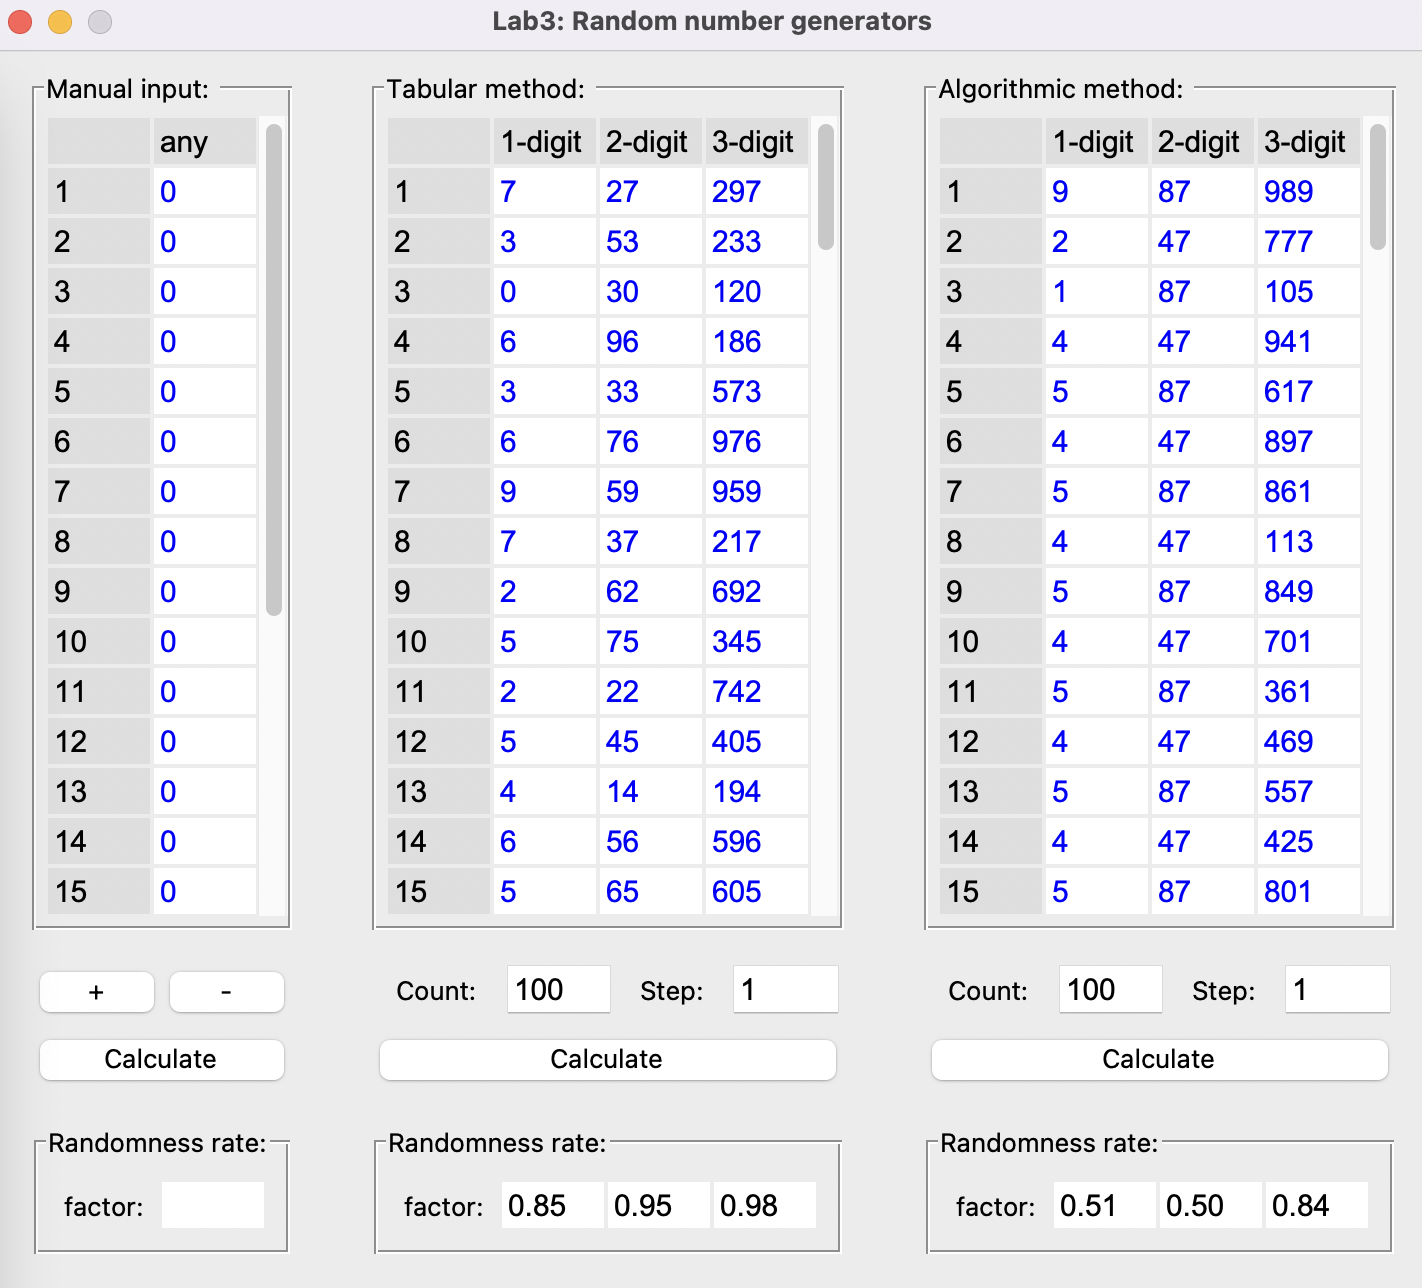
\includegraphics[width=1\textwidth]{inc/pic1.png}
	\caption{Пример работы программы --- 1}
	\label{fig:pic1}	
\end{figure}

\clearpage
На рисунке \ref{fig:pic2} изображен пример работы программы для последовательностей из 10000 элементов.
Заметим, что в данном случае были выбраны неоптимальные начальные значения для алгоритмического метода для последовательности одноразрядных чисел, полученных алгоритмическим методом. Полученная последовательность состоит из одного повторяющегося элемента, ввиду чего ее коэффициент случайности минимален. Для последовательностей двухразрядных и трехразрядных чисел, полученных алгоритмическим методом, были подобраны оптимальные значения, поэтому коэффициенты случайности для них велики. 
Коэффициенты случайности для всех трех последовательностей, полученных табличным методом, велики.

\begin{figure}[h!btp]
	\centering
	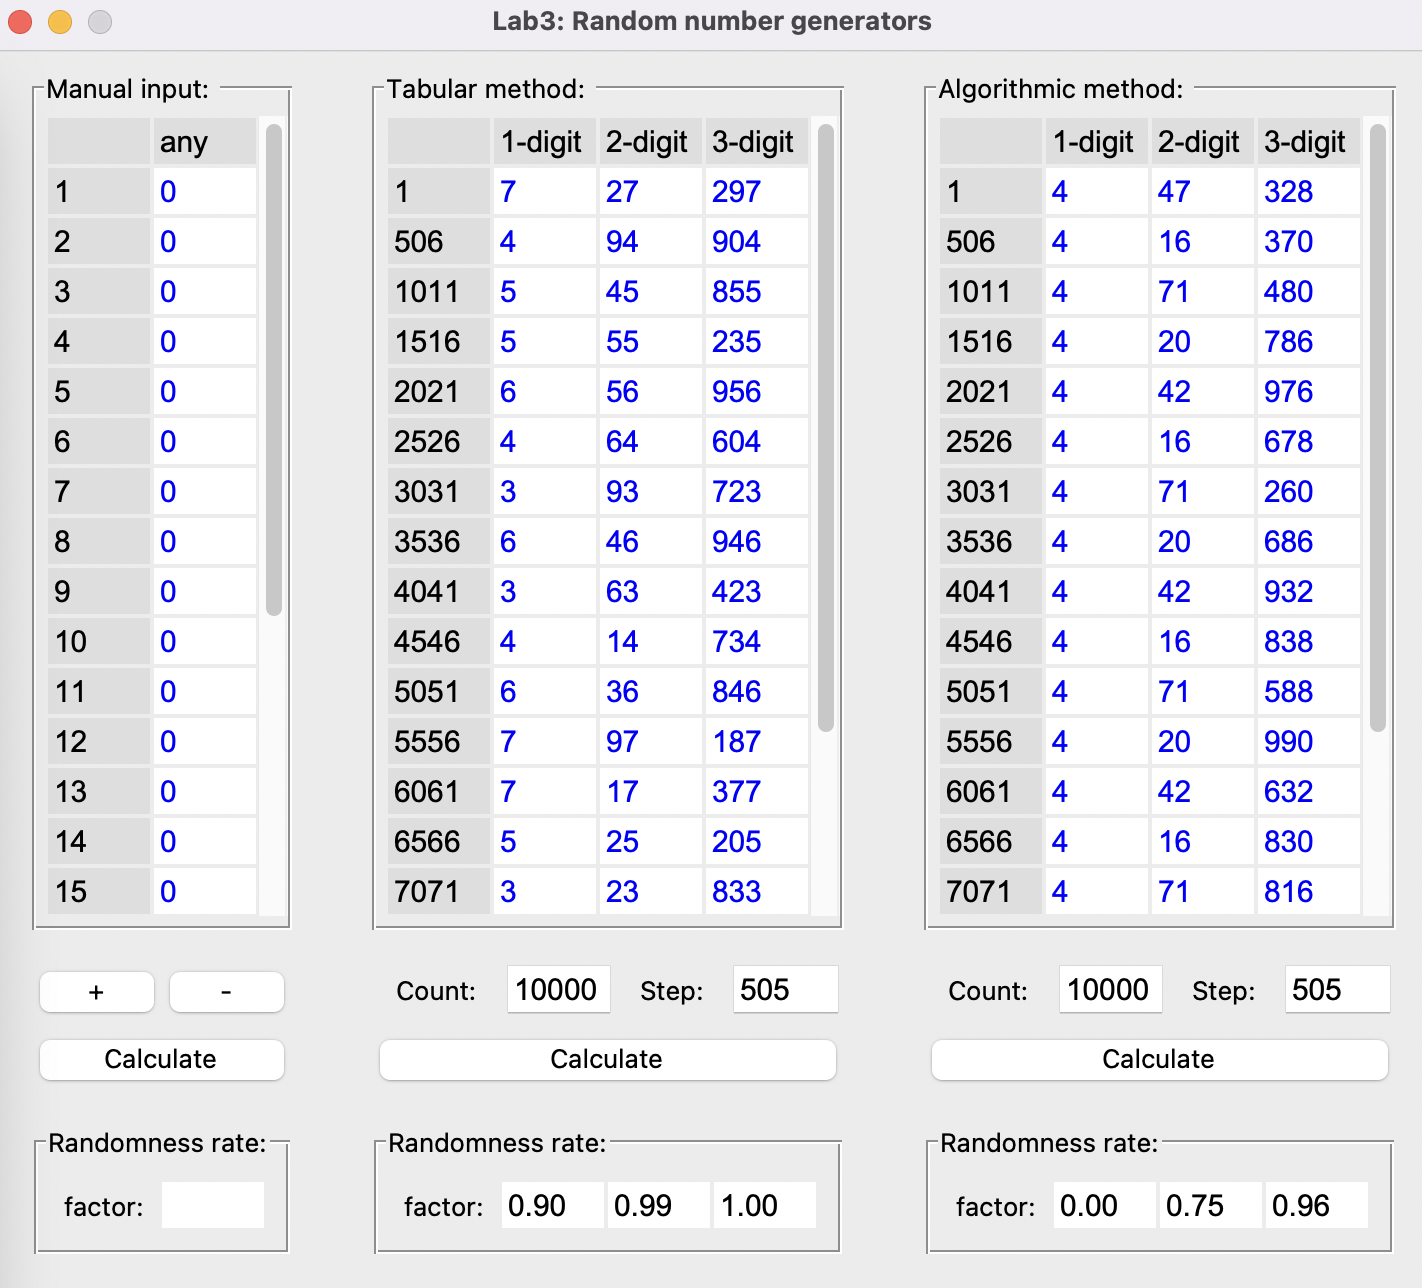
\includegraphics[width=1\textwidth]{inc/pic2.png}
	\caption{Пример работы программы --- 2}
	\label{fig:pic2}	
\end{figure}
\clearpage

На рисунке \ref{fig:pic3} изображен пример работы программы для последовательностей из 10000 элементов.
В данном случае были выбраны оптимальные начальные значения для всех трех последовательностей, полученных алгоритмическим методом. Коэффициент случайности для последовательности одноразрядных чисел несколько ниже двух других, т.к. в нем явно выражена периодичность.

\begin{figure}[h!btp]
	\centering
	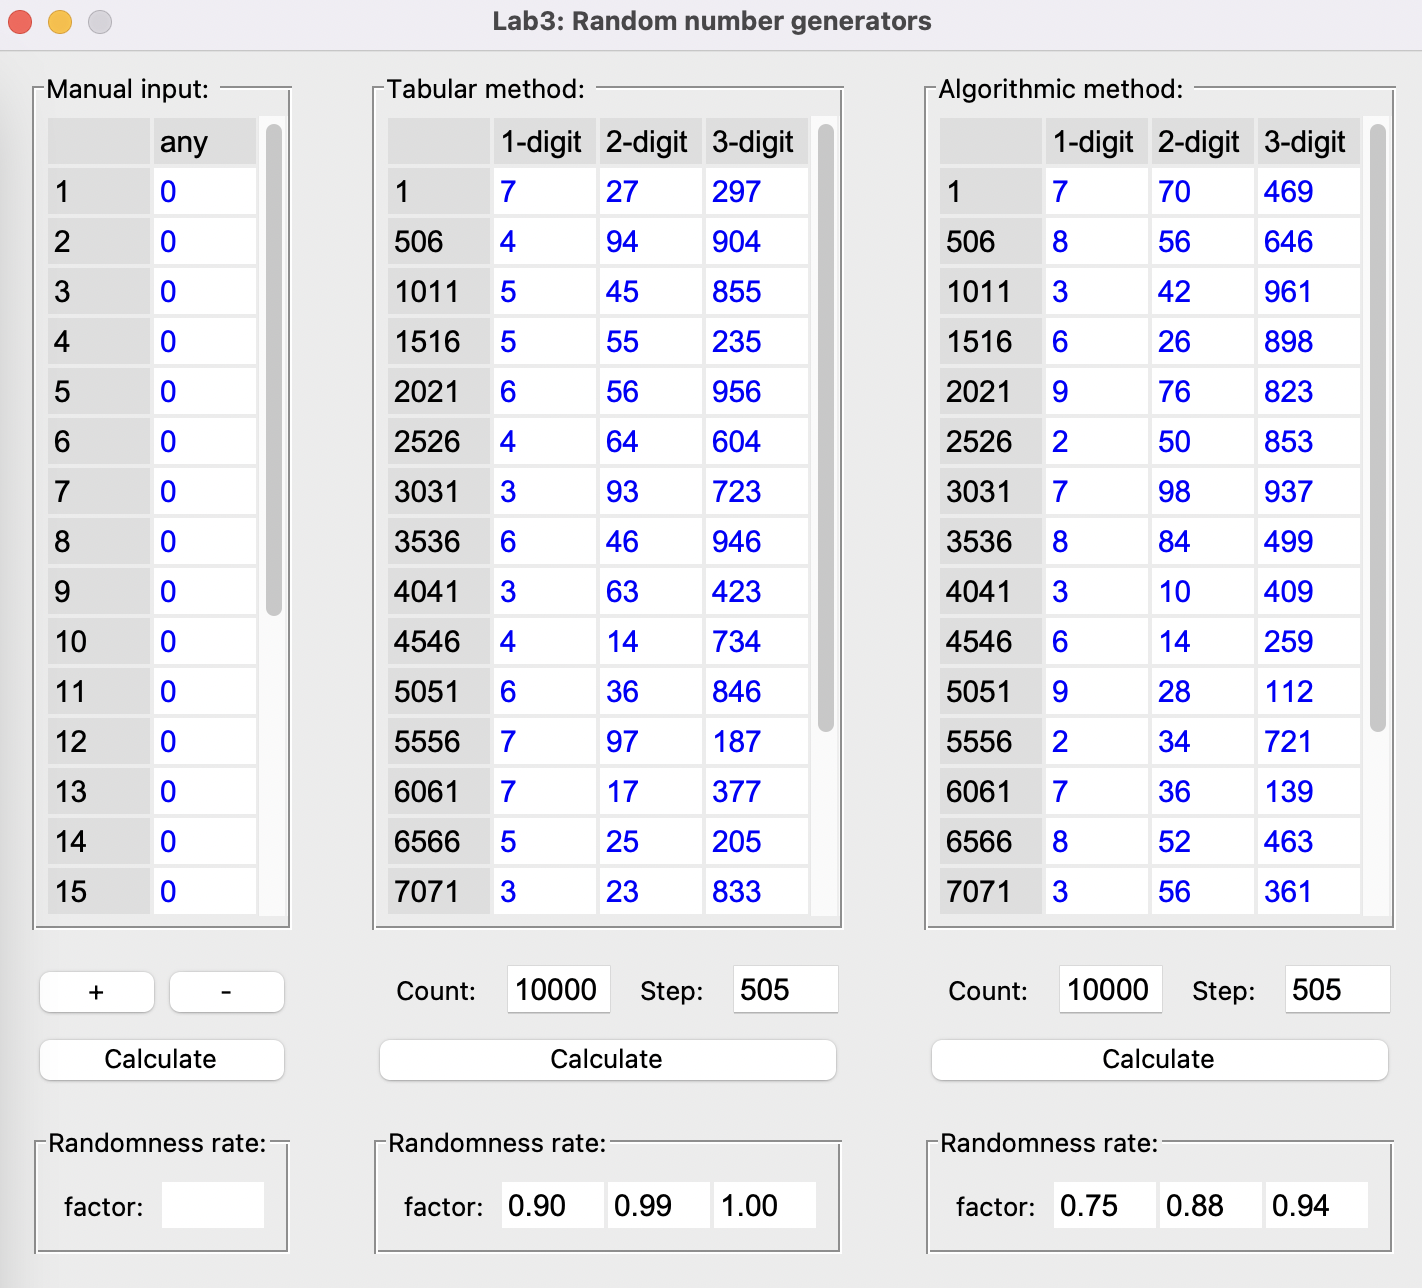
\includegraphics[width=1\textwidth]{inc/pic3.png}
	\caption{Пример работы программы --- 3}
	\label{fig:pic3}	
\end{figure}

\clearpage
На рисунке \ref{fig:pic4} изображен пример работы программы для последовательности, введенной вручную. Данная последовательность представляет собой арифметическую прогрессию с шагом 1, т.е. не является случайной. Коэффициент случайности имеет значение 0.5 ввиду того, что элементы в последовательности не повторяются, однако приращение между ними одинаково, т.е. присутствует связь между элементами.

\begin{figure}[h!btp]
	\centering
	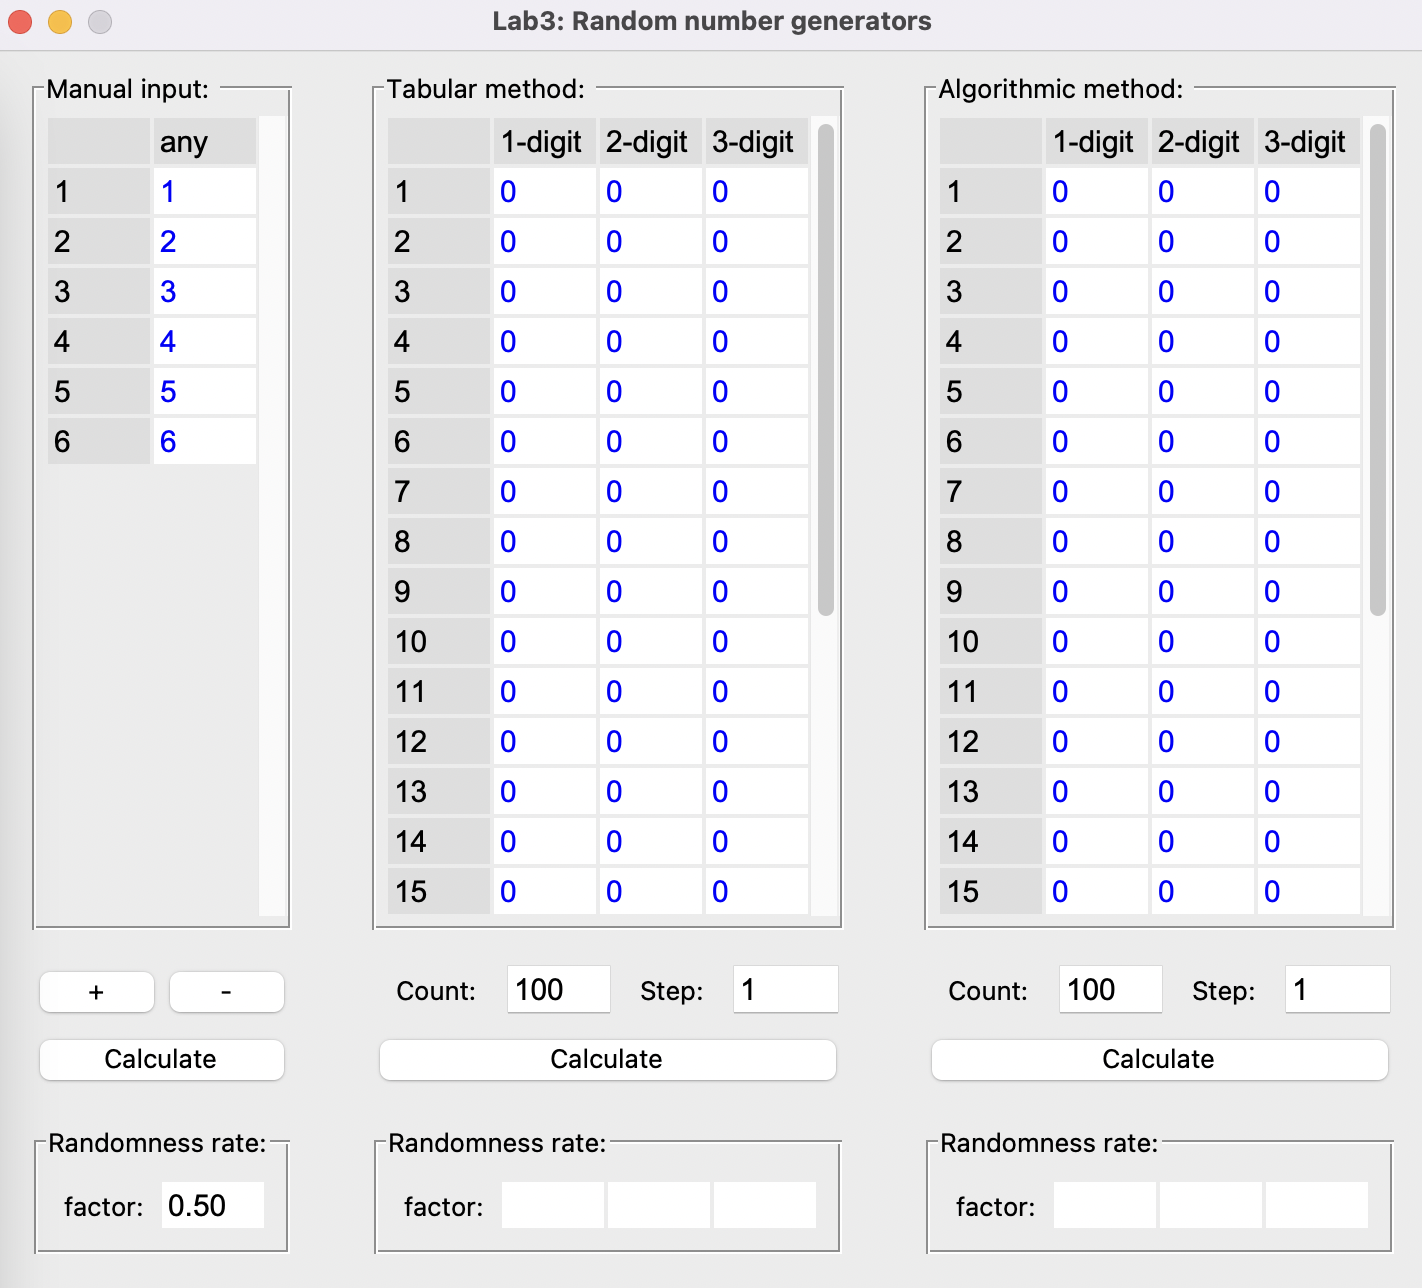
\includegraphics[width=1\textwidth]{inc/pic4.png}
	\caption{Пример работы программы --- 4}
	\label{fig:pic4}	
\end{figure}

\clearpage
На рисунке \ref{fig:pic5} изображен пример работы программы для последовательности, введенной вручную. Данная последовательность состоит из одного повторяющегося элемента, поэтому коэффициент случайности для нее получился минимальным.

\begin{figure}[h!btp]
	\centering
	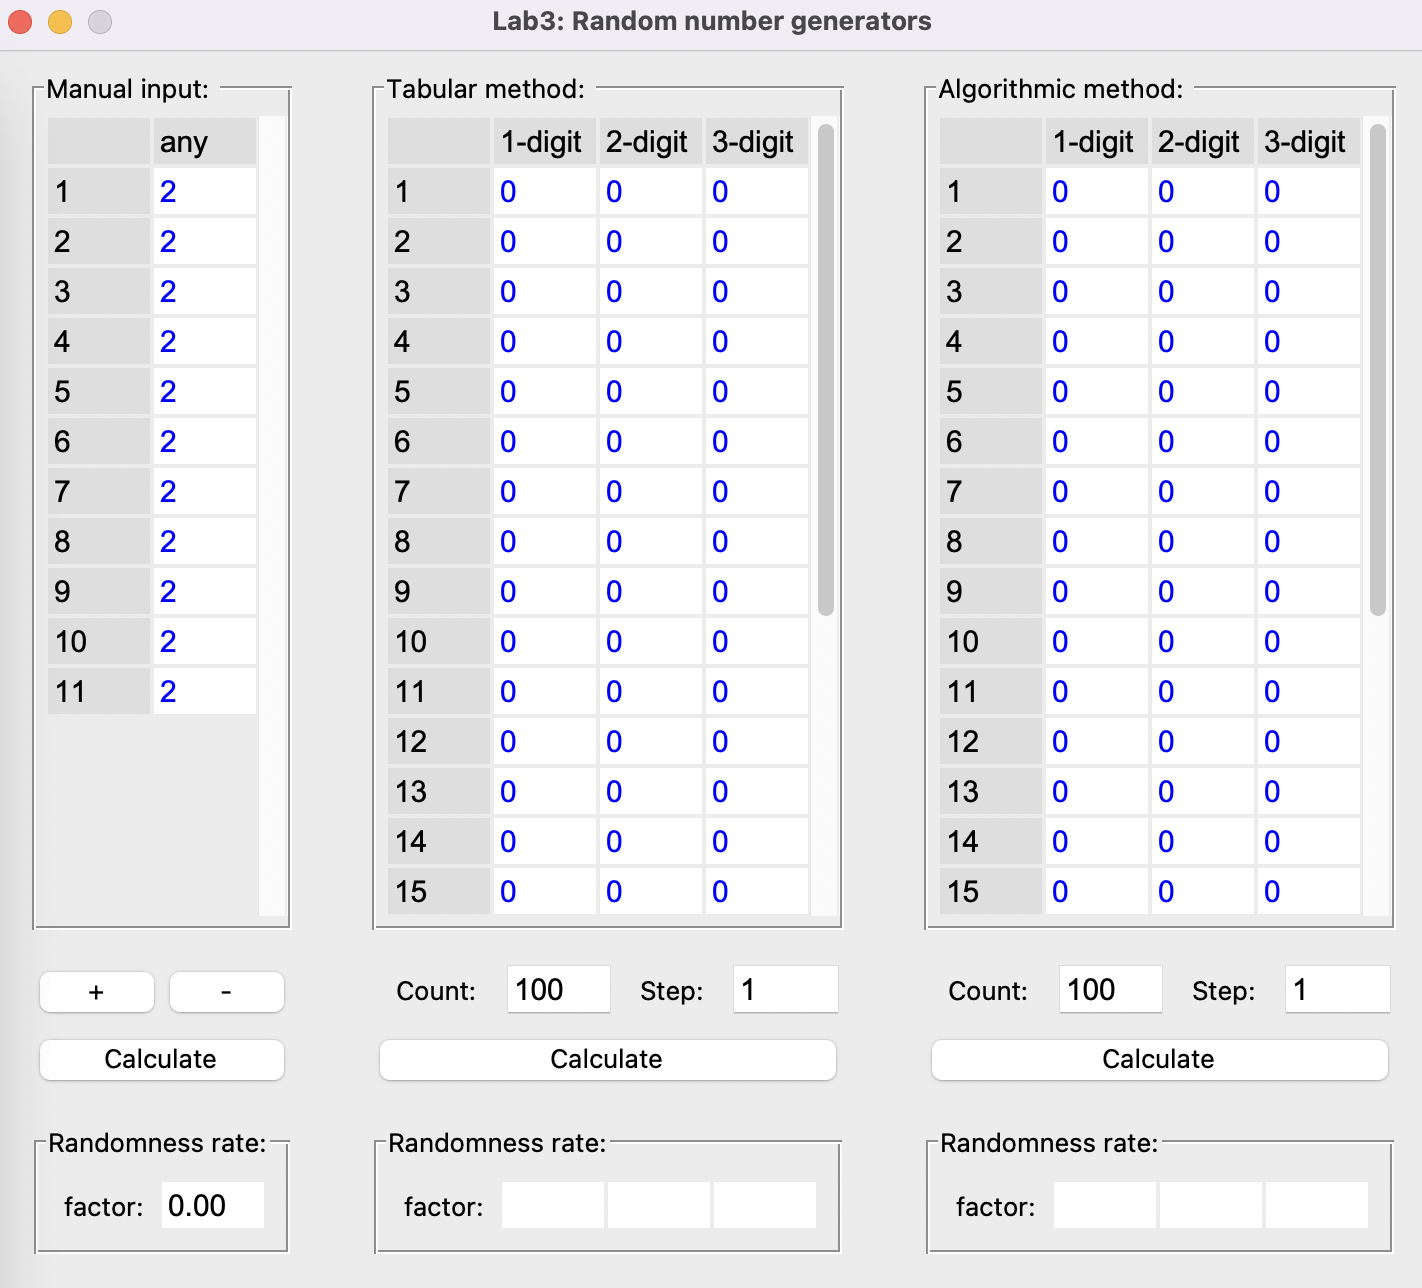
\includegraphics[width=1\textwidth]{inc/pic5.png}
	\caption{Пример работы программы --- 5}
	\label{fig:pic5}	
\end{figure}

\clearpage
На рисунке \ref{fig:pic6} изображен пример работы программы для последовательности, введенной вручную. Данная последовательность случайна, поэтому коэффициент случайности для нее велик.

\begin{figure}[h!btp]
	\centering
	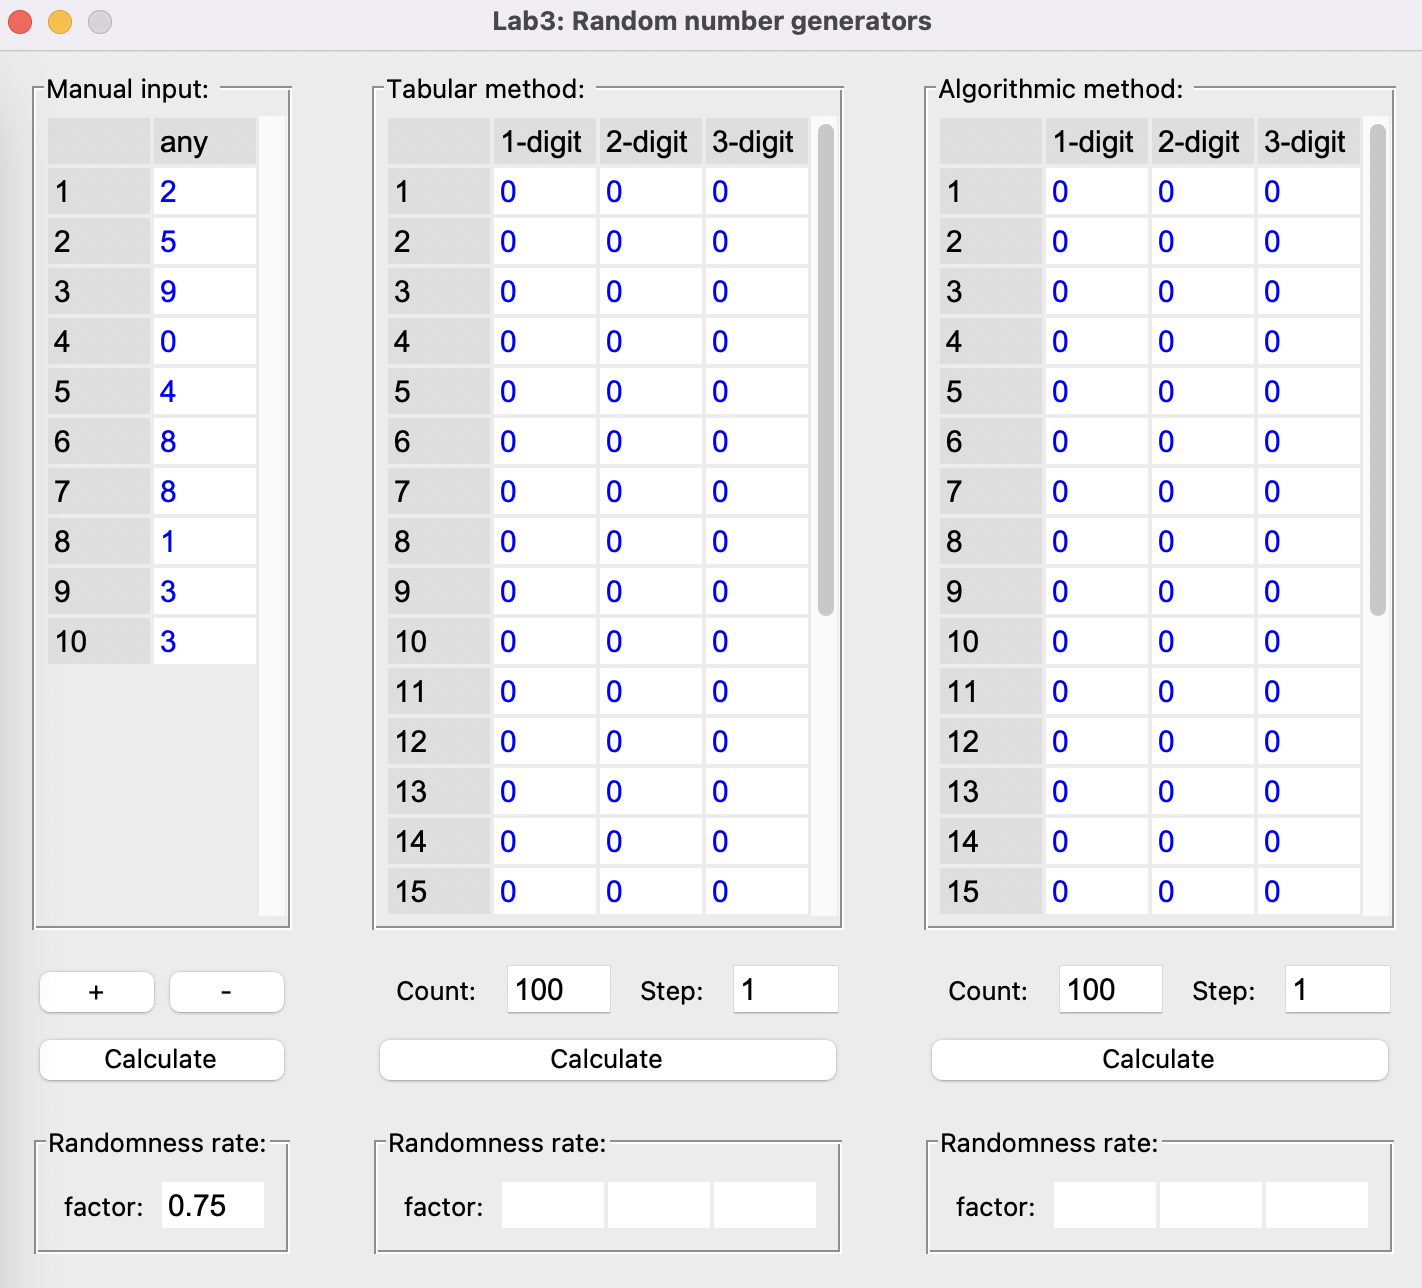
\includegraphics[width=1\textwidth]{inc/pic6.png}
	\caption{Пример работы программы --- 6}
	\label{fig:pic6}	
\end{figure}

\bibliographystyle{utf8gost705u}  % стилевой файл для оформления по ГОСТу
\bibliography{51-biblio}          % имя библиографической базы (bib-файла)
	
\end{document}
